\subsection{Introduction} \label{subsection:android-introduction}
%START TEXT INPUT
This is my real text! Rest might be copied or not be checked!
%START TEXT INPUT

%
Android is an open source Linux-based operating system running on a large set of touchscreen devices, wearables and many more\newline
Launched in 2007 by Google, it is designed to meet the limited computational capacity of a mobile device’s hardware. The principal processor of Android devices is the ARM platform for which the operating system is optimized\newline

AUFBAU ANDROID
\begin{figure}[h]
    \centering
    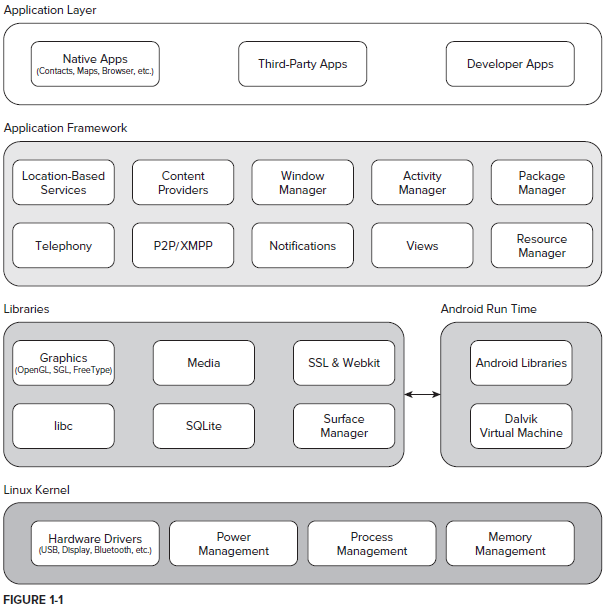
\includegraphics[width=0.8\textwidth]{data/stack.png}
    \caption{stack}
    \label{fig:stack}
\end{figure}
The underlying entity of the system is its kernel which bridges the hardware of the device and the remaining software components. Being a Linux-based kernel, it allows remote access to the device via a Linux shell as well as the execution of standard Unix commands.\newline
A level above is the Android Runtime, which will be explained closer\newline
At the same abstraction level as the virtual machine are the native libraries of the system. Written in C/C++, they permit low level interaction between the applications and the kernel through Java Native Interface (JNI)\newline
The next layer is the application framework which provides generic functionality to mobile software through Android’s  \gls{apig}.
The top layer of the Android OS stack is where custom applications are compiled, installed and executed.\newline
\cite{kovachevaMaster}
%


What is Android? Where is it used? When was it founded? Who does it belong to?\newline


platform developed by the "Android Open Source Project" -see- official website?\newline
currently one of the main operating systems for mobile devices -see- quelle\newline
focussed on simplicity for users, install of apps etc -see- quelle\newline
riesiger markt\newline
